\chapter{Background Theory}

\label{ch:background}
In this chapter, the background covered in this thesis is presented according to the following structure: in Section~\ref{ch3:dnn} and Section~\ref{ch3:bp}, we first briefly discuss deep neural network (DNN), back-propagation and optimisation methods. Then, in Section~\ref{ch3:rl}, some background to reinforcement learning (RL) is introduced. Next, in Section~\ref{ch3:policy-optim}, we discuss more details about policy optimisation in deep reinforcement learning (DRL) and related DRL algorithms that are covered in this thesis. Finally, in Section~\ref{ch3:dpp}, we introduce the fundamentals of determinantal point processes (DPPs).
%Finally, in Section~\ref{ch3:env}, we introduce the benchmark environments which are adopted to evaluate the proposed methods.

\section{Deep Neural Network in DRL}
\begin{figure}[h]
    \centering
    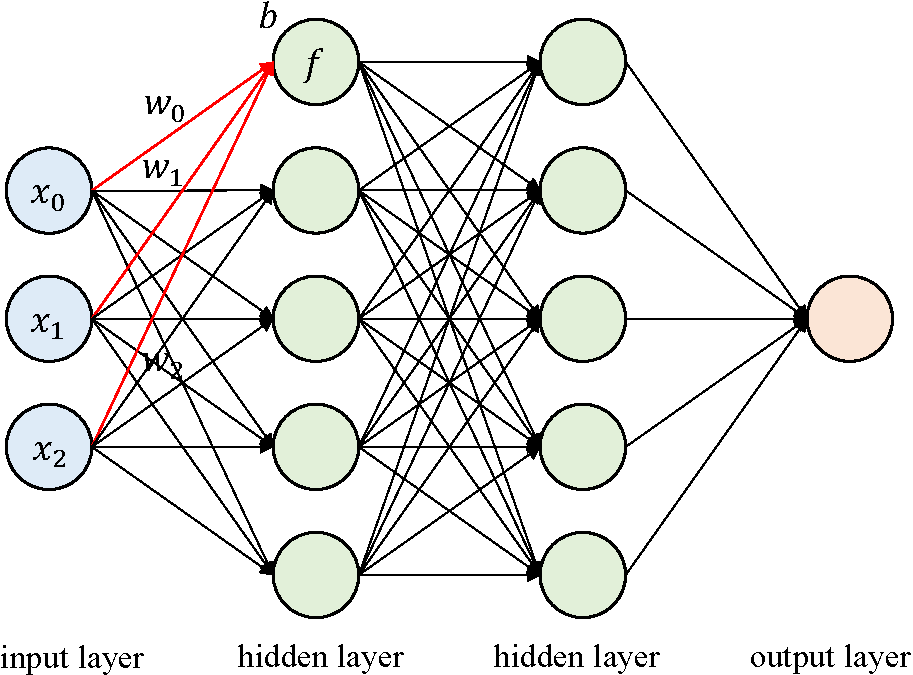
\includegraphics[width=0.7\textwidth]{figures/background/mlp_background.pdf}
    \caption{A simple structure of a multi-layer perceptron (MLP). It consists of an input layer, two hidden layers and an output layer. The highlighted lines (\textcolor{red}{red}) show the connection between a single neuron and its previous layer.}
    \label{fig:nn}
\end{figure}
\label{ch3:dnn}
\subsection{Multi-layer Perceptron}
Deep learning is based on research of artificial neural networks (ANNs). The structure of ANNs is inspired by animal brains, and mimics signal propagation between biological neurons. A feed-forward neural network (FFNN) or multi-layer perceptron (MLP) is a standard structure of ANN, and it consists of several neuron layers, which include an input layer, one or several hidden layers and an output layer (see Figure~\ref{fig:nn}). In each layer, there are multiple neurons, and each neuron is connected to those in the previous layer with corresponding weights $w_{i}$ and a bias $b$. For example, in Figure~\ref{fig:nn}, the transmission of the signal between the highlighted neuron and the previous layer can be expressed as:
\begin{equation}
    f = \sigma (w_{0}x_{0} + w_{1}x_{1} + w_{2}x_{2} + b)
\label{eq:nn_compute}
\end{equation}
here, $\sigma(\cdot)$ represents an activation function, such as a rectifier linear unit (ReLU)~\cite{nair2010rectified}, sigmoid$(\cdot)$ and tanh$(\cdot)$, which are used to add non-linearity to the network, because most real-world problems are nonlinear. The hidden layers in a neural network are used to learn various non-linear combinations of the input data, and the learned non-linear combinations are also called features. These features are the key factors to decide the prediction of the network.

The general forward propagation in an MLP that can be described as the following way. Firstly, the input layer receives the input data of a specific task. The input data can be a flattened image or the property of a house (e.g., the number of rooms, location, and area). Then, in each hidden layer, the output of each neuron is computed according to Equation~\eqref{eq:nn_compute}, and this computation proceeds from the first hidden layer to the last hidden layer. Finally, in the output layer, the output of the network can be the probability of each class in a classification task, the predicted value in a regression task, or the policy/predicted state value in a DRL task.

However, the initial parameters (i.e., weights and bias) of a FFNN may not fit a function for solving a specific task. Thus, the parameters need to be updated through a back-propagation method which is discussed in Section~\ref{ch3:bp}.
% CNN
\subsection{Convolutional Neural Network}
Multi-layer perceptrons (MLPs) are somewhat inefficient in dealing with computer vision tasks because of its fully connected structure. As the input size increases, the number of parameters (weight and bias) also increases. Convolutional neural network (CNN)~\cite{lecun1998gradient} alleviates this problem by using learnable kernels/filters, where each filter traverses the entire image. \td{CNNs are a strong inductive bias that reflects translation invariance of the physical world.} Compared with an MLP, the parameters of these kernels are shared, less, and easy to train. In previous works~\cite{krizhevsky2012imagenet,girshick2014rich,detone2016deep}, CNN has demonstrated its better feature representation ability than other hand-crafted methods, such as histogram of oriented gradient (HOG)~\cite{dalal2005histograms} and scale-invariant feature transform (SIFT)~\cite{lowe2004distinctive}. Nowadays, an increased number of powerful network structures have been proposed, such as the VGG network~\cite{simonyan2014very}, the residual network~\cite{he2016deep}, the dense network~\cite{huang2017densely}, and the capsule network~\cite{sabour2017dynamic}. These network structures improve state-of-the-art performance on various benchmark tasks~\cite{deng2009imagenet,everingham2010pascal}. In DRL, CNNs are regularly used to extract features from high-dimensional inputs (e.g., images) for further processing. In this thesis, as in many DRL studies, we put less effort into the design of the network structure.
%\td{[shifting and scaling in-variance makes CNN important]} 

\section{Back-propagation and Optimisation}
\label{ch3:bp}
Gradient descent~\cite{bottou2010large} is a common technique used to update the parameters of the deep neural network (DNN) to fit a model, and it relies on the gradient of an objective function/loss function with respect to the parameters of the network. The gradient can be calculated efficiently through using the back-propagation algorithm~\cite{kelley1960gradient}. In the forward propagation of an MLP with $N$ layers, the output of each hidden layer can be formulated as:
\begin{equation}
    \mathbf{f}_{i} = \sigma(\mathbf{W}_{i-1}\mathbf{f}_{i-1} + \mathbf{b}_{i-1}), \quad i = 1, 2, \cdots, N,
\end{equation}
where $\mathbf{f}_{i}$ is the output of the current hidden layer, $\mathbf{f}_{i-1}$ is the output of the previous hidden layer, and the input is $\mathbf{f}_{0}$; $\mathbf{W}_{i-1}$ and $\mathbf{b}_{i-1}$ are the weights and bias of the current layer, respectively. Then, in this example, we use the squared error as the loss function to calculate the gradient and update the parameters of the network:
\begin{equation}
    \min_{\bm{\theta}}\mathcal{L} = \norm{\mathbf{y} - \mathbf{f}_{N}(\mathbf{x};\bm{\theta})}^{2},
\end{equation}
where $\bm{\theta}$ is the collection of parameters of the network: $\{\mathbf{W_{0}}, \mathbf{b_{0}}, \mathbf{W_{1}}, \mathbf{b_{1}}, \cdots, \mathbf{W_{N-1}}, \mathbf{b_{N-1}}\}$, $\mathbf{y}$ is the ground truth value and $\mathbf{x}$ is the input data. To minimise the error between the ground truth and the prediction, we need to compute the partial derivatives of $\mathcal{L}$ with respect to the parameters $\bm{\theta}_{i}$ of each layer using the chain rule:
\begin{equation}
   \nabla_{\bm{\theta}_{i}}\mathcal{L} = \frac{\partial \mathcal{L}}{\partial \bm{\theta_{i}}} = \frac{\partial \mathcal{L}}{\partial \mathbf{f}_{N}} \frac{\partial\mathbf{f}_{N}}{\partial \mathbf{f}_{N-1}}\cdots \frac{\partial\mathbf{f}_{i+2}}{\partial \mathbf{f}_{i+1}} \frac{\partial\mathbf{f}_{i+1}}{\partial \bm{\theta}_{i}}.
\end{equation}

Once get the gradient $\nabla_{\bm{\theta}}\mathcal{L}$, the parameters $\bm{\theta}$ can be updated in the opposite direction of the gradient with a step size $\eta$ (i.e. learning rate) via gradient descent:
\begin{equation}
    \bm{\theta} \leftarrow \bm{\theta} - \eta\nabla_{\bm{\theta}}\mathcal{L}.
\end{equation}
However, gradient descent requires the calculation of the gradient over all samples, and it is inefficient when the number of samples is large. Stochastic gradient descent (SGD) reduces computational complexity by randomly splitting the entire samples into several minibatches, and each minibatch is comprised of one or more samples. Then, the gradient is computed over each minibatch samples to update the parameters. 
%Furthermore, SGD with momentum~\cite{qian1999momentum} can accelerate the convergence speed on top of standard SGD.
In this thesis, two variants of the SGD method are used to update the parameters of the network: root mean square propagation (RMSProp)~\cite{tieleman2012lecture} and Adam~\cite{kingma2014adam}.

Root mean square propagation (RMSProp) can adaptively adjust the learning rate for different parameters (i.e., per-parameter learning rate) to accelerate the convergence, the update rule can be written as:
\begin{align}
    \mathbf{v} &\leftarrow \beta \mathbf{v} + (1 - \beta)\nabla_{\bm{\theta}}\mathcal{L}\odot\nabla_{\bm{\theta}}\mathcal{L} \label{eq:squared_grad}\\
     \bm{\theta} &\leftarrow \bm{\theta} - \frac{\eta}{\epsilon+\sqrt{\mathbf{v}}}\odot\nabla_{\bm{\theta}}\mathcal{L} \label{eq:rmsprop_update}.
\end{align}
In Equation~\eqref{eq:squared_grad}, $\mathbf{v}$ is the moving average of the squared gradient, $\odot$ is the element-wise multiplication, and $\beta$ is the decay coefficient which indicates the ratio of history information used to compute the average value. In Equation~\eqref{eq:rmsprop_update}, $\epsilon$ is a small value to prevent division by zero, $\frac{1}{(\epsilon + \sqrt{\mathbf{v}})}$ is the weight to balance the learning rate for individual parameter, in doing so, the learning rate for large gradient will decrease to avoid exploding, and the learning rate for small gradient will increase to avoid vanishing.

Adam is a combination of momentum~\cite{qian1999momentum} and RMSProp, and it is the most popular optimiser in DRL community. The update rule of Adam is:
\begin{align}
    \mathbf{m} &\leftarrow \beta_{1} \mathbf{m} + (1 - \beta_{1})\nabla_{\bm{\theta}}\mathcal{L} \label{eq:momentum_adam}\\
    \mathbf{v} &\leftarrow \beta_{2} \mathbf{v} + (1 - \beta_{2})\nabla_{\bm{\theta}}\mathcal{L}\odot\nabla_{\bm{\theta}}\mathcal{L} \label{eq:squared_grad_adam}\\
     \bm{\theta} &\leftarrow \bm{\theta} - \frac{\eta}{\epsilon+\sqrt{\mathbf{v}}}\mathbf{m} \label{eq:adam_update}.
\end{align}
Equation~\eqref{eq:momentum_adam} is the momentum term, $\mathbf{m}$ is the running average of the gradient, and $\beta_{1}$ is the decay coefficient. The momentum term can correct the gradient in the right direction and thus accelerate the convergence. The other parts are similar to RMSProp.

\section{Reinforcement Learning}
\label{ch3:rl}
\subsection{Markov Decision Process}
\begin{figure}[h]
    \centering
    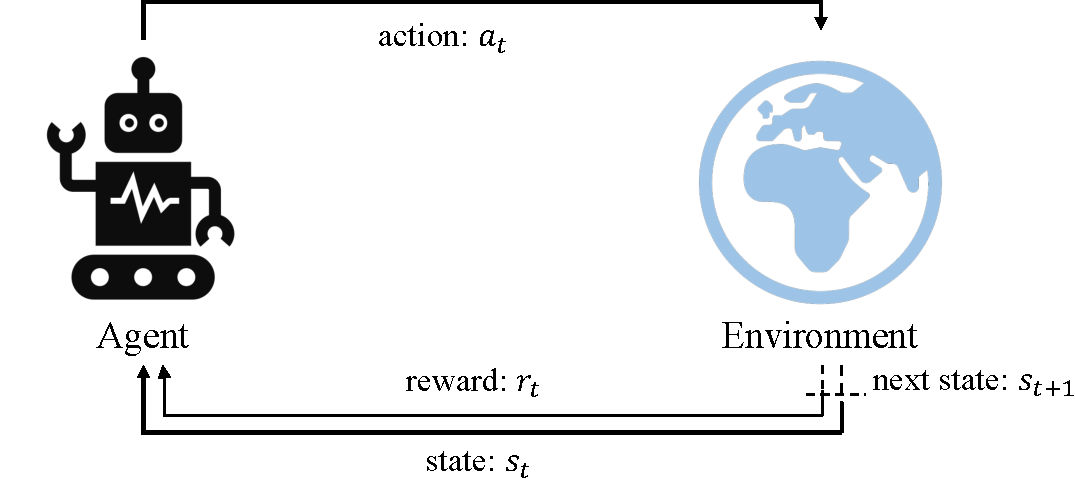
\includegraphics[width=0.8\textwidth]{figures/background/mdp_background.pdf}
    \caption{An overview of reinforcement learning (RL).}
    \label{fig:rl_desc}
\end{figure}
Reinforcement learning (RL) can be formulated under the framework of a Markov Decision Process (MDP); it is used to learn an optimal policy to solve sequential decision-making problems. The MDP is a mathematical framework which describes a fully observable environment in RL, and it is composed of a 5-tuple $<\mathcal{S}, \mathcal{A}, \mathcal{P}, \mathcal{R}, \gamma>$. $\mathcal{S}$ is a set of states, $\mathcal{A}$ is a set of actions, $\mathcal{P}$ is a transition probability/dynamics function: $p(s_{t+1}|s_{t},a_{t})$ which only depends on the current state and action, $\mathcal{R}$ is a reward function, and $\gamma$ is a discount factor. At each timestep $t$, a state $s_{t}\in\mathcal{S}$ is received by an agent from the environment (see Figure~\ref{fig:rl_desc}). An action $a_{t}\in\mathcal{A}$ is sampled by the agent according to its policy $\pi(a_{t}|s_{t})$. Then, the next state $s_{t+1}$ and reward $r_{t}$ are provided to the agent according to the transition function and the reward function. The goal of the RL is to have the agent learn a policy that maximises the expected return $\mathbb{E}_{\pi}[G_{t}]$~\cite{sutton2018reinforcement}:
\begin{equation}
\centering
    G_{t} =\sum_{k=0}^{T-1}\gamma^{k}r_{t+k}.
\label{eq:acc_reward_func}
\end{equation}
Here, the discount factor $\gamma$ exponentially downplays the influence of future rewards. {In a robot manipulation task, the state $s_{t}$ can be the velocity and position of each joint of a robot arm. The action $a_{t}$ can be the velocities of actuators (control signals)} and the reward $r_{t}$ might be calculated based on the distance between the gripper of the robot arm and the target position.

\subsection{Goal-Oriented Reinforcement Learning}
\label{ch3:goal_rl}
The purpose of goal-oriented RL or multi-goal RL is to acquire a policy that can achieve different goals within the environment. 
%Universal Value Function Approximators (UVFA) is proposed to solve such 
In this thesis, the experiments in Chapter~\ref{ch:esil} and Chapter~\ref{ch:dtgsh} follow the terminology suggested by OpenAI~\cite{plappert2018multi}, in which the possible goals are drawn from a goal space $\mathcal{G}$, and the goal being pursued does not influence the environment dynamics. Two types of goal are recognised. One is the desired goal $g\in \mathcal{G}$, which is the target position {or state}, and may be different for different episodes. Within a single episode, $g$ is constant.  The second type of goal is the achieved goal $g^{ac}_{t}$, which is the achieved state in the environment (e.g., the position of an object), and this is considered to be different at each timestep in an episode. In an episode, each transition can be represented as $(s_t|\langle g, g^{ac}_{t} \rangle, a_t, r_t, s_{t+1}|\langle g, g^{ac}_{t+1} \rangle)$, where $s_t$ indicates a state, $a_t$ indicates an action and $r_t$ indicates a~reward; $\langle \, , \rangle$ is simply used to represent the grouping of goals.

\begin{figure}[h]
    \centering
    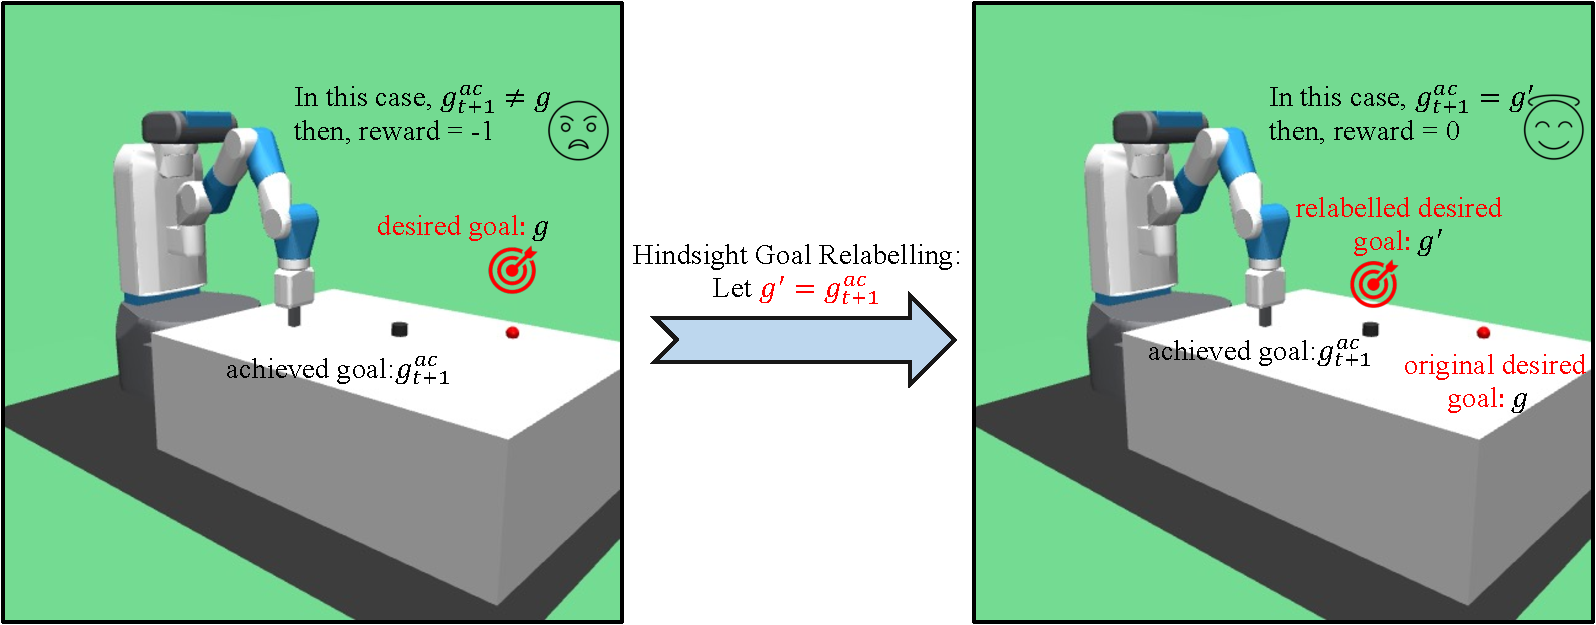
\includegraphics[width=0.85\textwidth]{figures/background/her_background.pdf}
    \caption{A brief illustration of the hindsight goal relabelling in a robotic manipulation task~\cite{plappert2018multi}. In this task, the agent needs to control the gripper to hit the puck and make it slide to a specific position, where the achieved goal is the position of the puck and the desired goal is the target position (the red spot).}
    \label{fig:her_back}
\end{figure}
In sparse reward settings, an agent will only get non-negative rewards when the desired goal $g$ is achieved. The sparse reward function can be defined as:
\begin{equation}
r_{t}\left(g^{ac}_{t+1}, g\right):=
\begin{cases}
0& \text{if $\left\|g^{ac}_{t+1} - g\right\|\leq\epsilon$}\\
-1& \text{otherwise},
\end{cases}
\label{eq:sparse_reward}
\end{equation}
where $\epsilon$ is a threshold value, used to identify if the agent has achieved the goal. {However, the desired goal, $g$, might be difficult to reach during training. Thus, hindsight experiences~\cite{andrychowicz2017hindsight} (see Figure~\ref{fig:her_back}) are created through replacing the original desired goal $g$ with the current achieved goal $g_{t+1}^{ac}$ to augment successful samples, and then reward $r_{t}$ can be recomputed according to Equation~\eqref{eq:sparse_reward}. The modification of the desired goal can be denoted as $g^\prime$ and transitions from hindsight experiences can be represented as $(s_t|\langle g^\prime, g^{ac}_{t} \rangle, a_t, r_t, s_{t+1}|\langle g^\prime, g^{ac}_{t+1} \rangle)$.} {Intuitively, introducing $g^\prime$ serves a useful purpose in the early stages of training; taking, for example, a robot reaching task, the agent has no prior ``concept" of how to move its effector to a specific location in space. Thus, even these original failed episodes contain valuable information for ultimately learning a useful control policy for the original, desired goal $g$.}

\section{Policy Optimisation in DRL}
\label{ch3:policy-optim}
Policy optimisation in DRL can be roughly classified into three categories: 1) value-based methods (see Section~\ref{ch3:value-based}), 2) policy-based methods (see Section~\ref{ch3:policy-based}), and 3) the actor-critic methods, which are the combination of value-based and policy-based methods (see Section~\ref{ch3:actor-critic}).

\subsection{Value-based Methods}
\label{ch3:value-based}
% value based
Value-based methods aim to learn a state or state--action value function instead of an explicit policy. The value function can evaluate the quality of a given state or the quality of an action performed at a given state. Then, the agent can select an action according to the corresponding estimate. This section will discuss how to derive a policy through the value function.

%and for a given state, the agent selects an action according to the prediction of the value function. When the values of states are predicted (i.e. state value function), the agent can select the action towards the next state with the highest state value. When the values of each action are estimated (i.e. state-value function), the agent selects the action with the highest value.

The state value function $V_{\pi}(s_{t})$ under a policy $\pi$ is the expected return when starting from the state $s_{t}$, and can be defined as:
\begin{equation}
\centering
    V_{\pi}(s_{t}) = \mathbb{E}_{\pi}[G_{t}] = \mathbb{E}_{\pi}\biggr[\sum_{k=0}^{T-1} \gamma^{k}r_{t+k}\biggr].
\end{equation}
Through the Bellman equation, the state value function can be rewritten as the combination of the immediate reward, $r_{t}$, and the discounted state value of the next state, $V_{\pi}(s_{t+1})$:
\begin{equation}
\centering
     V_{\pi}(s_{t}) = \mathbb{E}_{\pi}[r_{t} + \gamma V_{\pi}(s_{t+1})].
\end{equation}
% state-action value function
\td{Apart from estimating the state value,} we can also predict the value of a particular state--action pair, denoted as $Q_{\pi}(s_{t},a_{t})$, and this has a similar definition to the state value function:
\begin{equation}
\centering
     Q_{\pi}(s_{t},a_{t}) = \mathbb{E}_{\pi}[G_{t}] = \mathbb{E}_{\pi}\biggr[\sum_{k=0}^{T-1} \gamma^{k}r_{t+k}\biggr].
\end{equation}
The state--action value function $Q_{\pi}(s_{t},a_{t})$ is also called the Q-value function. Similarly, the Q-value function can also be expressed in a recursive form:
\begin{equation}
\centering
     Q_{\pi}(s_{t},a_{t}) = \mathbb{E}_{\pi}[r_{t} + \gamma Q_{\pi}(s_{t+1}, a_{t+1})].
\end{equation}
Next, the optimal policy can be derived using these value functions. In RL, the agent aims to follow the policy that can achieve more accumulated rewards from the environment. Thus, an optimal policy $\pi_{*}$ is defined as the policy that achieves the maximum/optimal state value function, $V_{*}(s_{t})$:
\begin{equation}
    V_{*}(s_{t}) = \max_{\pi}V_{\pi}(s_{t}).
\end{equation}
Similarly, an optimal policy is also defined as the policy that achieves the maximum/optimal Q-value function $Q_{*}(s_{t},a_{t})$:
\begin{equation}
    Q_{*}(s_{t},a_{t}) = \max_{\pi}Q_{\pi}(s_{t},a_{t}).
\end{equation}
Particularly, the optimal policy $\pi_{*}$ can be achieved through this optimal Q-value function directly:
\begin{equation}
    \pi_{*}(s_{t}) = \argmax_{a_{t}} Q_{\pi}(s_{t}, a_{t}).
\end{equation}
Therefore, finding the optimal Q-value function is equivalent to finding the optimal policy. The optimal Q-value function can be reorganised using the Bellman optimality equation:
% bellman optimality equation
\begin{equation}
\centering
     Q_{*}(s_{t},a_{t}) = \mathbb{E}[r_{t} + \gamma\max_{a_{t+1}} Q_{*}(s_{t+1}, a_{t+1})].
\end{equation}
Q-learning~\cite{watkins1992q} is a tabular and iterative update method to solve this equation. In Q-learning, the state--action pairs and corresponding Q-values are stored in a table. For a given state, the action is selected with an exploration strategy (e.g., $\epsilon$-greedy) to observe the next state and the reward, and the Q-value of the current state is updated via:
\begin{equation}
    Q_{\pi}(s_{t}, a_{t}) \leftarrow Q_{\pi}(s_{t}, a_{t}) + \alpha(r_{t} + \gamma\max_{a_{t+1}}Q_{*}(s_{t+1}, a_{t+1}) - Q_{\pi}(s_{t}, a_{t})),
\end{equation}
where $\alpha$ is the learning rate, and this process is repeated until the estimated Q-value converges to the optimal Q-value.

\subsubsection{Function Approximator and Deep Q-Network}
\td{Q-learning in its tabular form}, is impractical to scale to tasks with high-dimensional states, such as playing a video game using images as inputs. The Deep Q-Network (DQN)~\cite{mnih2015human} overcomes this difficulty by combining deep learning and Q-learning. In DQN, instead of updating the Q-value function in a table, a convolutional neural network (CNN) is leveraged to approximate the Q-value function from a stack of images directly:
\begin{equation}
    Q(s_{t},a_{t};\theta) \approx Q^{*}(s_{t},a_{t}),
\end{equation}
here, $\theta$ represents the parameters of a main network. During training, the agent collect samples from the environment with the $\epsilon$-greedy exploration strategy, and each transition ($s_{t}$, $a_{t}$, $r_{t}$, $s_{t+1}$) is stored in a replay buffer $\mathcal{D}$. The replay buffer is designed to reuse past experiences. When updating the parameters $\theta$, a minibatch of transitions is sampled from the replay buffer to minimise the mean squared error (MSE) between the target Q-value and the estimated Q-value using gradient descent methods (e.g., SGD):
\begin{equation}
    \min_{\theta}\mathcal{L} = \mathbb{E}_{(s_{t}, a_{t}, r_{t}, s_{t+1})\sim\mathcal{D}}[(Q(s_{t}, a_{t};\theta) - (r_{t} + \gamma\max_{a_{t+1}}Q(s_{t+1}, a_{t+1};\theta^{-})))^{2}],
\end{equation}
here, $\theta^{-}$ is the parameters of a target network, which is used to estimate the target Q-value. The target network has the same structure as the main network, and its parameters are copied from the main network at each fixed step. The target network is also used to stabilise the training. 

\subsection{Policy-based Methods}
\label{ch3:policy-based}
% policy based
Policy-based methods learn a policy function $\pi(a_{t}|s_{t};{\theta})$, parameterised by $\theta$, and it directly maps a given state $s_{t}$ to an action $a_{t}$. In discrete control tasks, the output of the policy function is a categorical distribution over the action space. In continuous control tasks, the output of the policy function is often the parameters of a Gaussian distribution. During training, the actions are sampled from the corresponding distribution for exploration. In policy-based methods, the optimal parameters $\theta$ can be found by maximising expected returns in the environment:
\begin{align}
    \max_{\theta}J & = \mathbb{E}_{\pi_{\theta}}[G_{t}] \\
                   & = \sum_{s_{t}\in\mathcal{S}}d(s_{t})\sum_{a_{t}\in\mathcal{A}}\pi(a_{t}|s_{t};\theta)G_{t},
\end{align}
where $d(s_{t})$ is the stationary distribution in the Markov chain under the policy $\pi_{\theta}$. In order to maximise the expected returns, we need to increase the probability of the actions which lead to higher returns, and the gradient of the objective function can be expressed as:
\begin{align}
    \nabla_{\theta} J &= \sum_{s_{t}\in\mathcal{S}}d(s_{t})\sum_{a_{t}\in\mathcal{A}}\nabla_{\theta}\pi(a_{t}|s_{t};\theta)G_{t} \\
    &= \sum_{s_{t}\in\mathcal{S}}d(s_{t})\sum_{a_{t}\in\mathcal{A}}\pi(a_{t}|s_{t};\theta)\frac{\nabla_{\theta}\pi(a_{t}|s_{t};\theta)}{\pi(a_{t}|s_{t};\theta)}G_{t}\\
    &= \sum_{s_{t}\in\mathcal{S}}d(s_{t})\sum_{a_{t}\in\mathcal{A}}\pi(a_{t}|s_{t};\theta)\nabla_{\theta}\log\pi(a_{t}|s_{t};\theta)G_{t} \\
    &=\mathbb{E}_{\pi_{\theta}}[\nabla_{\theta}\log\pi(a_{t}|s_{t};\theta)G_{t}], \label{eq:reinforce}
\end{align}
where Equation~\eqref{eq:reinforce} is also known as REINFORCE~\cite{williams1992simple}, and the parameters are updated via gradient ascent. In practice, the return value $G_{t}$ is calculated using Monte Carlo methods, leads to a high variance in the estimated gradient, and slows the convergence of the policy function. In order to alleviate the above shortcomings, actor-critic methods are introduced. 

\subsection{Actor-Critic Methods}
\label{ch3:actor-critic}
Actor-critic methods combine both policy-based methods and value-based methods. The actor is the policy function $\pi(a_{t}|s_{t};\theta)$ to generate an action for a given state. The critic is the value function $V(s_{t};\psi)$ or Q-value function $Q(s_{t},a_{t};\psi)$ to evaluate the quality of a state or a state--action pair and thus guides the training of the actor. To reduce the variance in policy-based methods, a common practice is to subtract a baseline from the estimated return $G_{t}$~\cite{sutton2018reinforcement}. In REINFORCE, the state value predicted by the critic $V(s_{t};\psi)$ is selected as the baseline:
\begin{equation}
    A(s_{t}, a_{t}) = G_{t} - V(s_{t};\psi),
\end{equation}
where $A(s_{t}, a_{t})$ is an advantage function, and the gradient of the policy function can be rewritten as:
\begin{equation}
    \nabla_{\theta} J = \mathbb{E}_{\pi_{\theta}}[\nabla_{\theta}\log\pi(s_{t},a_{t};\theta)A_{t}].
\end{equation}
The critic can also be updated through minimising the MSE error between the return value $R_{t}$ and the estimated state value $V(s_{t};\psi)$:
\begin{equation}
    \min_{\psi}\mathcal{L} = \mathbb{E}[(G_{t} - V(s_{t};\psi))^2].
    \label{eq:mse}
\end{equation}
This actor-critic method is called advantage actor-critic (A2C). For more efficient training, A2C also utilises multiple CPU workers to collect samples from separate environments to update the actor and the critic~\cite{mnih2016asynchronous}. However, A2C does not perform well in continuous control tasks. In this paper, two actor-critic DRL methods -- deep deterministic policy gradient (DDPG)~\cite{lillicrap2015continuous} and proximal policy gradient (PPO)~\cite{schulman2017proximal} -- are adopted as the base algorithms to address the continuous control tasks.

\subsubsection{Deep Deterministic Policy Gradient}
Unlike the previous policy gradient methods (e.g., A2C) which output a probability distribution over the action space, DDPG outputs an action from the actor directly:
\begin{equation}
    a_{t} = \pi(s_{t}; \theta),
\end{equation}
and the critic is a Q-value function $Q(s_{t}, a_{t};\psi)$ to guide the learning of the actor. During training, noise is added to the action $a_{t}$ to help exploration, and the collected transitions are stored in a replay buffer $\mathcal{D}$. For each update iteration, a minibatch sized transitions is sampled to update the actor and the critic. The actor aims to maximise the expected returns $\mathbb{E}[Q(s_{t}, a_{t};\psi)|_{a_{t}=\pi(s_{t};\theta)}]$ and the gradient of the objective function can be estimated using chain rule:

\begin{align}
    \nabla_{\theta}J &\approx\mathbb{E}_{s_{t}\sim\mathcal{D}}[\nabla_{\theta}Q(s_{t}, a_{t};\psi)|_{a_{t}=\pi(s_{t};\theta)}]\\
    & = \mathbb{E}_{s_{t}\sim\mathcal{D}}[\nabla_{a_{t}}Q(s_{t}, a_{t};\psi)|_{a_{t}=\pi(s_{t};\theta)} \nabla_{\theta}\pi(s_{t};\theta)].
\end{align}
The update of the critic is similar to DQN which minimises the MSE between the target Q-vaule and the estimated Q-value:
\begin{equation}
    \min_{\psi}\mathcal{L} = \mathbb{E}_{(s_{t}, a_{t}, r_{t}, s_{t+1})\sim\mathcal{D}}[(Q(s_{t}, a_{t};\psi) - (r_{t} + \gamma Q(s_{t+1}, \pi(s_{t+1};\theta^{-});\psi^{-})))^{2}],
\end{equation}
where $\theta^{-}$ and $\psi^{-}$ are the parameters of the target actor network and the target critic network, respectively. These two target networks are updated toward the parameters of the two main networks slowly using a moving average scheme:
\begin{align}
    \theta^{-} &= \tau\theta^{-} + (1-\tau)\theta\\
    \psi^{-} &= \tau\psi^{-} + (1-\tau)\psi
\end{align}
here, $\tau\in$(0,1) is a coefficient that decides the updating speed of the target networks. 

\subsubsection{Proximal Policy Optimisation}
Before introducing proximal policy optimisation (PPO), we first review its forerunner -- trust region policy optimisation (TRPO)~\cite{schulman2015trust}. When updating the policy network using gradient-based methods, an inappropriate step size (i.e. learning rate) may lead to a worse policy, and the samples collected by this updated policy may interfere with the further policy improvements. In TRPO, when maximising the expected return of a policy network, an extra Kullback-Leibler (KL) divergence term is used to guarantee a promising step size and to restrict the policy update in a specific (trust) region. This constrained objective function can be expressed as:
\begin{align}
   & \max_{\theta} J = \mathbb{E}_{\pi_{\theta_{old}}}\biggr[\frac{\pi(a_{t}|s_{t};\theta)}{\pi(a_{t}|s_{t};\theta_{old})}A(s_{t},a_{t})\biggr] \\
   & \text{subject to} \enspace \mathbb{E}_{\pi_{\theta_{old}}}[\text{KL}[\pi(\cdot|s_{t};\theta_{old}), \pi(\cdot|s_{t};\theta)]] \leq \delta,
\end{align}
where $\theta$ and $\theta_{old}$ are the parameters of the current policy network and the old policy network, respectively, and $\delta$ is a value to limit changes between policies. This objective function can be solved via the method of Lagrange multipliers. In addition, a line search method can be used to estimate an appropriate step size, with the conjugate gradient method being used to estimate the gradient. Although TRPO achieves great performance in continuous control tasks, it is not flexible to be implemented and it performs poorly on tasks with high-dimensional inputs, such as playing Atari games.

Proximal policy optimisation (PPO) provides a simplified solution of TRPO with a clipped objective function to constrain changes of policy during an update:
\begin{equation}
\centering
\max_{\theta}J = \mathbb{E}_{\theta}\biggr[\min\bigg (\frac{\pi(a_{t}|s_{t};\theta)}{\pi(a_{t}|s_{t};\theta_{old})},
	\clip \bigg(\frac{\pi(a_{t}|s_{t};\theta)}{\pi(a_{t}|s_{t};\theta_{old})}, 1-\epsilon, 1+\epsilon \bigg)\bigg )A(s_t, a_t)\biggr],
\label{eq:standard_ppo}
\end{equation}
where $\epsilon$ represents the clipping ratio. In practice, PPO makes the implementation more accessible and improves the performance in tasks with high-dimensional inputs.

\section{Determinantal Point Processes}
\label{ch3:dpp}
A determinantal point process (DPP)~\cite{kulesza2012determinantal} is a stochastic process that characterises a probability distribution over sets of points using the determinant of some function. In machine learning, it is often used to quantify the diversity of a subset, with applications such as video~\cite{mahasseni2017unsupervised} and document summarisation~\cite{hong2014improving}.

Formally, for a discrete set of points $\mathcal{Y}=\{\mathbf{x}_{1}, \mathbf{x}_{2}, \cdots, \mathbf{x}_{N}\}$, a point process $\mathcal{P}$ is a probability measure over all $2^{|\mathcal{Y}|}$ subsets. $\mathcal{P}$ is a DPP if a random subset $\mathbf{Y}$ is sampled with probability:
\begin{equation}
    \mathcal{P}_{L}(\mathbf{Y}=Y) = \frac{\text{det}(\mathbf{L}_{Y})}{\sum_{Y'\subseteq \mathcal{Y}} \text{det}(\mathbf{L}_{Y'})} = \frac{\text{det}(\mathbf{L}_{Y})}{\text{det}(\mathbf{L}+\mathbf{I})},
\end{equation}
where $Y\subseteq \mathcal{Y}$, $\mathbf{I}$ is the identity matrix, $\mathbf{L} \in \mathbb{R}^{N\times N}$ is the positive semi-definite DPP kernel matrix, and $\mathbf{L}_{Y}$ is the sub-matrix with rows and columns indexed by the elements of the subset $Y$. 

The kernel matrix $\mathbf{L}$ can be represented as the Gram matrix $\mathbf{L} = \mathbf{X}^{T}\mathbf{X}$, where each column of $\mathbf{X}$ is the feature vector of an item in $\mathcal{Y}$. The determinant, $\text{det}(\mathbf{L}_{Y})$, represents the (squared) volume spanned by vectors $\mathbf{x}_{i}\in Y$. From a geometric perspective, feature vectors that are closer to being orthogonal to each other will have a larger determinant, and vectors in the spanned subspace are more likely to be sampled: $\mathcal{P}_{L}(\mathbf{Y}=Y) \propto \text{det}(\mathbf{L}_{Y})$. Using orthogonality as a measure of diversity, we leverage DPPs to sample diverse trajectories and goals in Chapter~\ref{ch:dtgsh}. In Chapter~\ref{ch:daim}, we use DPPs to model an intrinsic motivation, which aims to encourage the agent to explore novel states in the environment.